
\documentclass[promaster]{thesis-uestc}

\title{面向数据价值共享的激励机制设计与实现}{An Incentive Mechanism for Data Sharing}

\author{罗通}{Luo Tong}
\advisor{罗光春\chinesespace 教授}{Dr. Guangchun Luo}
\school{计算机科学与工程学院\chineseleftparenthesis网络空间安全学院\chineserightparenthesis}{School of Computer Science and Engineering}
\major{计算机技术}{Computer Technology}
\studentnumber{201722060929}

\begin{document}

\makecover

\begin{chineseabstract}
为了适应日益增长的宽带信号和非线性系统的工程应用,用于分析瞬态电磁散射问题的时域积分方程方法研究日趋活跃。本文以时域积分方程时间步进算法及其快速算法为研究课题,重点研究了时间步进算法的数值实现技术、后时稳定性问题以及两层平面波算法加速计算等,主要研究内容分为四部分。

……

\chinesekeyword{时域电磁散射,时域积分方程,时间步进算法,后时不稳定性,时域平面波算法}
\end{chineseabstract}

\begin{englishabstract}
With the widespread engineering applications ranging from broadband signals and non-linear systems, time-domain integral equations (TDIE) methods for analyzing transient electromagnetic scattering problems are becoming widely used nowadays. TDIE-based marching-on-in-time (MOT) scheme and its fast algorithm are researched in this dissertation, including the numerical techniques of MOT scheme, late-time stability of MOT scheme, and two-level PWTD-enhanced MOT scheme. The contents are divided into four parts shown as follows.

\englishkeyword{time-domain electromagnetic scattering, time-domain integral equation (TDIE), marching-on in-time (MOT) scheme, late-time instability, plane wave time-domain (PWTD) algorithm}
\end{englishabstract}

\thesistableofcontents

\thesischapterexordium

\section{研究工作的背景与意义}

计算电磁学方法\citing{wang1999sanwei, liuxf2006, zhu1973wulixue, chen2001hao, gu2012lao, feng997he}从时、频域角度划分可以分为频域方法与时域方法两大类。频域方法的研究开展较早,目前应用广泛的包括:矩量法(MOM)\citing{xiao2012yi,zhong1994zhong}及其快速算法多层快速多极子(MLFMA)\citing{clerc2010discrete}方法、有限元(FEM)\citing{wang1999sanwei,zhu1973wulixue}方法、自适应积分(AIM)\citing{gu2012lao}方法等,这些方法是目前计算电磁学商用软件\footnote{脚注序号“\ding{172},……,\ding{180}”的字体是“正文”,不是“上标”,序号与脚注内容文字之间空1个半角字符,脚注的段落格式为:单倍行距,段前空0磅,段后空0磅,悬挂缩进1.5字符;中文用宋体,字号为小五号,英文和数字用Times New Roman字体,字号为9磅;中英文混排时,所有标点符号(例如逗号“,”、括号“()”等)一律使用中文输入状态下的标点符号,但小数点采用英文状态下的样式“.”。}(例如:FEKO、Ansys 等)的核心算法。由文献\cite{feng997he,clerc2010discrete,xiao2012yi}可知

\section{国内外研究历史与现状}
时域积分方程方法的研究始于上世纪60 年代,C.L.Bennet 等学者针对导体目标的瞬态电磁散射问题提出了求解时域积分方程的时间步进(marching-on in-time, MOT)算法。

\section{本文的主要贡献与创新}
本论文以时域积分方程时间步进算法的数值实现技术、后时稳定性问题以及两层平面波加速算法为重点研究内容,主要创新点与贡献如下:

\section{本论文的结构安排}
本文的章节结构安排如下:

\section{本章小结}

\chapter{相关理论基础}
此部分主要抄书

\section{基本概念}
hello

\subsection{激励相容}
DSIC

\subsection{最优拍卖}
Ideal

\section{麦尔森引理}

\section{算法机制设计}

    \subsection{背包拍卖}

    \subsection{显示定理}

\section{税收最大化拍卖}

\section{简单近似拍卖}

\section{多变量环境}

\section{预算受限的机制设计}

\section{无金钱机制设计}

\section{动态规划}

\subsection{背包问题}

\section{本章小结}

\chapter{简单可并行计算下的机制}

\section{引言}
\subsection{原位计算}

原位计算的介绍及总体基本场景描述待补

\subsection{信誉系统}
待补,之前看过的文章有。此部分也可能放在第四章

\section{基本假设}
在简单可并行计算下的机制建立之前,首先给出相关合理假设。

假设1:参与者是有限理性的个体,总是执行理性条件下最大化各自效用函数的策略,且不存在共谋

假设2:除参与者对原位计算任务代价的内心估值为私密知识以外,其余均为公共知识,为平台方和其它参与者所知。

\section{基础模型}

\subsection{模型定义}
\label{jichumoxingdingyi}

机制中以虚拟代币作为货币。机制中有$n$个参与者$\mathbf{agent}$可以进入原位计算任务$T$的竞拍环节。原位计算任务$T$共需要$datademand$单位的计算。对于$1\leq i\leq n$,参与者$agent_i$可以针对任务书$T$提供$datacount_i$单位的原位计算任务。
而参与者$agent_i$拥有私密值$0 \leq val_i = INCENT-cost_i$,$INCENT$是平台方给予胜出者的每单位计算任务的固定奖赏,由平台方或者原位计算任务发起者确定\footnote{本文中不特意区分平台方与计算任务发起者,因为他们可能是同一角色}。$0 \leq cost_i \leq INCENT$,否则,参与者$agent_i$应当退出此次竞拍来避免自己受损。 于是,$val_i$表示$agent_i$对购买每单位原位计算任务带来的真实价值。其$val_i$只对参与者$agent_i$可见,平台方及其余参与者不可见。在机制中,每个参与者会提交自己的标的$b_i$,形成标的向量$\mathbf{bid}$。分配函数$\mathbf{allocation}(\mathbf{bid})$也是一个向量,表示了机制对参与者分配的原位计算任务数量。$agent_i$的效用函数定义为准线性函数$utility_i = val_i*allocation_i-payment_i$。总社会福利$\mathbf{SW}$定义为$\sum_{i=1}^n{val_i*allocation_i}$,其是所有参与者的效用函数与平台方收益的总和。即:$\mathbf{SW} = \sum_{i=1}^n{utility_i}+\sum_{i=1}^{n}{payment_i}$

\subsection{模型求解}
本文的目标是设计一种参与者具有占优策略的拍卖机制。由显示定理可知,对于任意一个参与者总是具有占优策略的机制$M$,总是存在一个等价的直接显示(direct-revelation)占优策略激励相容(DSIC)机制$M'$。因此,本文在DSIC机制的范围中寻找合适的解。而在前述基础模型定义中,参与者的私密值仅为其对购买原位计算任务的收益真实估值$val_i$,且效用函数为准线性函数。这属于单变量环境,需要麦尔森引理来主导机制设计的流程。

假设所有参与者已经真实地表达原位计算任务的估值,并给出标的,即$\mathbf{bid} = \mathbf{val}$。 此时对于平台方来说,社会福利最大化等价于最优化问题\ref{jichumoxing}。

\begin{align}
    \label{jichumoxing}\max_{\vec{allocation}} \quad&\sum_{i=1}^{n}{bid_i*allocation_i}\\
    s.t                     \quad& 0\leq allocation_i\leq datacount_i,\quad allocation_i = {0,1,2...}\notag\\
                            \quad& \sum_{i=1}^{n}{allocation_i} = datademand\notag 
\end{align}

给出贪心算法:\footnote{本文中数组下标均从1开始计数}
\footnote{可以通过first和second来分别指代二元组的第一、二关键字}时间复杂度$O(n)$

\begin{algorithm}[H] 
    \KwIn{$\mathbf{datacount},\mathbf{bid},datademand$}
    \KwOut{$\mathbf{allocation}$}
    $i \leftarrow 1$\;
    $total \leftarrow datademand $\;
    对二元组序列$list = \{(bid_j,j)|1 \leq j \leq n\}$以第一关键字进行降序排列,第一关键字相同的情况下,以第二关键字升序排列\;
    \While{total > 0}{
        \If{i > n}{
            datademand单位的计算任务无法被分配完毕,返回错误信息。
            break\;
        }
        $temp \leftarrow \min(total,\quad datacount_{list[i].second})$\;
        $total \leftarrow total - temp$\;
        $allocation_i \leftarrow temp$\;
        $i \leftarrow i + 1$\;
    }
\caption{贪心算法求解基础模型}
\label{tanxin}
\end{algorithm}

\begin{theorem}
算法\ref{tanxin}是问题\ref{jichumoxing}的解。
\end{theorem}

\begin{proof}
    算法\ref{tanxin}的思想是在供应$datademand$有限的情况下,优先满足代价估值$bid_i$更大的参与者的需求。假设存在一个更优解$S^1(SW^1 > SW)$与该思想相悖。即存在$1 \leq i \neq j \leq n,bid_i > bid_j$, 使得$allocation_i < datacount_i \text{, } allocation_j > 0$。不妨将分配给参与者$agent_j$的$temp = min(datacount_i - allocation_i,allocation_j)$单位计算任务重新分配给参与者$agent_i$,得到解$S^2$,此时新的社会福利$SW^2= SW^1- temp*bid_j + temp*bid_i=SW^1+temp*(bid_i-bid_j)$,由前述条件可知,$temp > 0$且$bid_i - bid_j > 0$。易得,$SW^1<SW^2 $。继续对$S^2$执行以上流程,直到前提条件不满足。此时,解$S^n$优先满足代价估值更大的参与者的需求。由贪心算法可知$SW^n = SW$,则$SW^1<SW^2...<SW^n=SW$,这与假设不符。故不存在上述更优解。
\end{proof}

分配函数已经确定,为了应用麦尔森引理确定价格函数,需要首先分析分配函数关于标的$bid_i$的单调性。

\begin{theorem}
    对于任意参与者$agent_i$以及任意$\mathbf{bid_{-i}}$\footnote{表示除$bid_i$分量以外的总标的向量},算法\ref{tanxin}所示分配规则$allocation_i(z,\mathbf{bid_{-i}})$是关于$agent_i$的标的$z$的单调不减函数。
\end{theorem}

\begin{proof}
   在保持其余标的不变的情况条件下,若$agent_i$的标的$z$变大,则其在算法\ref{tanxin}中list序列中的排位只会更加靠前,从而获得更高优先级的分配权力。而算法的不确定性已经由第二关键字排序消除。
\end{proof}



\begin{figure}[h]
    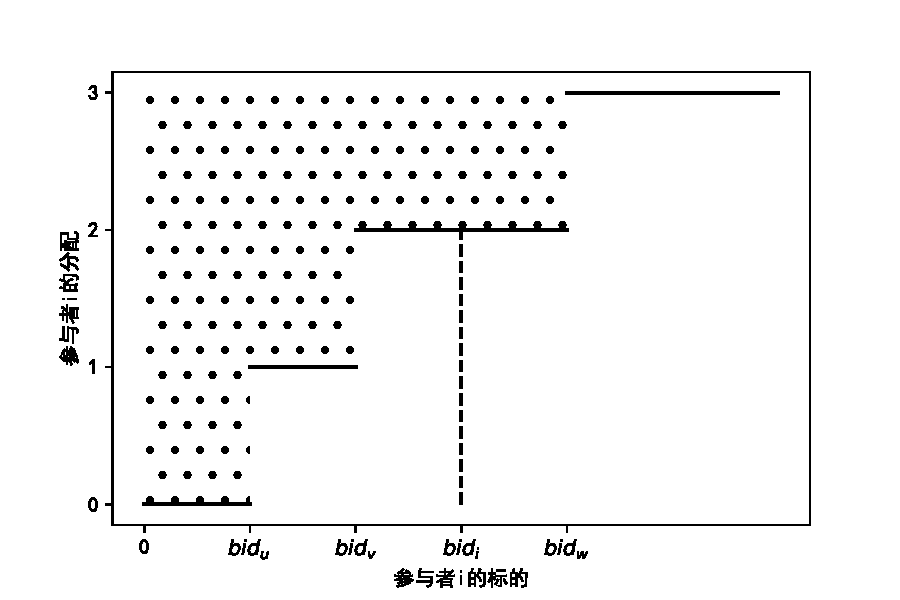
\includegraphics{pic/tanxin_allocation.pdf}
    \caption{贪心算法分配函数示例}
    \label{tanxin_allocation}
\end{figure}

不失一般性,$allocation_i(z,\mathbf{bid_{-i}})$函数图像如图\ref{tanxin_allocation}所示。
根据麦尔森引理,阴影部分面积即为$agent_i$向平台方支付的报酬。由图像可知,需要求解出这些阶跃变化值。根据贪心算法的流程,假设已知根据$\mathbf{bid}$降序排列的$\mathbf{datacount}$前缀和数组$\mathbf{prefix}$,则可以迭代求出这些阶跃值,从而求得阴影部分总面积。其余$agent$的代价计算亦然。总体$\mathbf{payment}$计算具体细节如算法\ref{tanxin_zhifu}所示,算法时间复杂度$O(n^2)$。

\begin{algorithm}[H]
    \KwIn{$\mathbf{datacount},\mathbf{bid},datademand$}
    \KwOut{$\mathbf{payment}$}
    运行算法\ref{tanxin},获得list\;
    \tcp{根据标的排序求count的各前缀和}
    prefix 置为初始值为0的数组\;
    \For{$i = 1$ \KwTo $n$}
    {
        \If{i > 1}{
            $prefix[i] \leftarrow prefix[i-1]$\;
        }
        $prefix[i]  += datacount_{list[i].second}$\;
    }
    \tcp{求每个参与者的支付$payment_i$}
    \For{$i = 1$ \KwTo $n$}
    {
        $payment_{list[i].second} \leftarrow 0$\;
        \tcp{ind存储遍历下标}
        $ind \leftarrow i + 1$
        \tcp{y存储当前分配值}
        \eIf{$i = 1$}
        {
            $y \leftarrow min(datademand,datacount_{list[i].second})$\;
        }{
        $y \leftarrow min(max(datademand - prefix[i-1],0),datacount_{list[i].second})$\;
        }
        \While{$ind \leq n$ 且 $y > 0$}
        {
            $newy \leftarrow min(max(datademand - prefix[ind]+ datacount_{list[i].second},0),datacount_{list[i].second})$\;
            $payment_{list[i].second} += (y - newy)*list[ind].first$\;
            $y \leftarrow newy$\;
            $ind += 1$\;
        }
    }
\caption{贪心算法求解基础模型的支付流程}
\label{tanxin_zhifu}
\end{algorithm}

\section{多重指标限制问题}
\label{dptou}
\subsection{问题描述及定义}
    原位计算任务竞拍场景中,平台方或者任务提交方对于任务购买方存在总体偏好设置或者限制条件。例如:平台方可以出于总体计算结果来源异构性等需求要求竞拍胜出者的数量不能超过某给定阈值;或者要求原位计算任务$T$的总体响应时间不能大于给定目标值。在本场景中,参与者会被赋予不同的信誉等级及可靠性评估。而平台方也可以根据自己对任务难易程度的估量,制定不同的限制条件。假设限制指标集$Limit$是有限集。本文中使用表\ref{zhibiao}所示指标作为分析。

\newcommand{\tabincell}[2]{\begin{tabular}{@{}#1@{}}#2\end{tabular}} %放在导言区

\begin{table}[h]
\caption{限制指标集}
\label{zhibiao}
\begin{tabular}{cp{10em}cc}
    \toprule
    指标名称& 描述&符号&产生方式\\
    \midrule
    一级参与者的数量阈值&来自信誉系统&$Parti_1$&由平台方或任务方确定\\
    二级参与者的数量阈值& 同上&$Parti_2$&由平台方或任务方确定\\
    三级参与者的数量阈值& 同上&$Parti_3$&由平台方或任务方确定\\
    总体响应时间和&各个胜出者完成来自任务$T$所指派计算花费的时间总和&TIME&由平台方或任务方确定\\
    计算需求量&&datademand&任务$T$固有属性\\
    \bottomrule
\end{tabular}
\end{table}

上述指标集中,前三项来自于对参与者的信誉等级及可靠性评估。前三项指标是同类指标,以第一项为例,它意味着平台方要求任务$T$的胜出者中一级参与者刚好有$Parti_1$个。第四项指标衡量了原位计算任务$T$的总体完成效率。$TIME$值越小,意味平台方对于任务的响应要求越高,对于拍卖环节的限制也就更强。第五项$datademand$是来自于原位计算任务本身的需求,机制需要尽可能使$datademand$被满足,这里也将其视为平台方对原位计算任务分配的限制指标之一。
\subsubsection{形式化定义}
\label{dpdingyi}
在\ref{jichumoxingdingyi}节所示基础上引入上述指标集限制条件。$level_i\in {1,2,3}$为$agent_i$的信誉及可靠性评估。对于$1\leq j \leq 3$,胜出者集合中第$j$级参与者数量$=parti_j$。$timeperunit_i$是$agent_i$关于$任务T$完成每单位
计算任务所花费的时间。$transmitcost_i$是$agent_i$向平台方提交结果数据所花费的平均时间,主要由网络时延、吞吐量等因素决定。分配规则需要满足时效性要求指标:$\sum_{i=1}^{n}{timeperunit_i*allocation_i+\mathbf{I}(allocation_i > 0)*transmitcost_i} < TIME$
\footnote{$\mathbf{I}(\text{表达式}) = \begin{cases}{}
        0&,\text{表达式为假}\\
        1&,\text{表达式为真}
        \end{cases}$
}%,$timeperunit_i$和$transmitcost_i$的定义见\ref{dpdingyi}节。}
社会福利$SW$的定义仍然不变。
假设所有参与者已经真实地表达原位计算任务的估值,并给出标的,即$\mathbf{bid} = \mathbf{val}$,此时对于平台方来说,社会福利最大化等价于最优化问题\ref{dpmoxing}
\begin{align}
    \label{dpmoxing}\max_{\vec{allocation}} \quad&\sum_{i=1}^{n}{bid_i*allocation_i}\\
    s.t\quad& 0\leq allocation_i\leq datacount_i,\quad allocation_i = {0,1,2...}\notag\\
        \quad& \sum_{i=1}^{n}{allocation_i} = datademand\notag\\
        \quad& \left(\sum_{i=1}^{n}{timeperunit_i*allocation_i+\mathbf{I}(allocation_i > 0)*transmitcost_i}\right) < TIME\notag\\
        \quad& \left(\sum_{i=1}^{n}{\mathbf{I}(allocation_i > 0,level_i = j)}\right)=parti_j, j = {1,2,3}\notag
\end{align}

\subsection{模型求解}
最优化问题\ref{dpmoxing}是一个NP-hard问题,此处尝试以动态规划的方式进行求解。拟定6维状态$dp[i,j,a,b,c,t]$,表示考虑前$i$个参与者,刚好分配$j$单位原位计算任务,其中一级参与者$a$个,二级参与者$b$个,三级参与者$c$个,最多花费$t$单位总时间,所能够获得的最大收益。通过枚举分配给$agent_i$的计算任务数量,可以得到状态转移方程\ref{dpfangcheng}。

\begin{gather}
\label{dpfangcheng}  
dp[i,j,a,b,c,t] = max
\begin{cases}
1 \leq k \leq datacount_i \\
\text{If} \quad level_i = 1,\\
dp[i-1,j-k,a-1,b,c,t-k*timeperunit_i-transmitcost_i]+ k*bid_i,\\
\text{If}\quad level_i = 2,\\
dp[i-1,j-k,a,b-1,c,t-k*timeperunit_i-transmitcost_i]+ k*bid_i,\\
\text{If} \quad level_i = 3,\\
dp[i-1,j-k,a,b,c-1,t-k*timeperunit_i-transmitcost_i]+ k*bid_i,\\
\text{all condition},\\
dp[i-1,j,a,b,c,t]
\end{cases}\\
dp[0,0...datademand,0...parti_1,0...parti_2,0...parti_3,0...TIME] =-\infty \notag\\
dp[0,0,0,0,0,0...TIME] = 0 \notag
\end{gather}
上述转移方程中,值得一提的是状态的初始化方法。考虑最优化问题\ref{dpmoxing}的限制条件可知,只有总体响应时间和是不等式限制,其余四项限制指标均等式。这可以通过设置初始状态的合法性来解决。如\ref{dpfangcheng}所示,在限制指标张成的五维空间中,仅有关于运行时间的一维子空间\footnote{此处并非完整定义的子空间}被赋予合法性。其余非法状态置$-\infty$。当限制指标集扩展时,针对不同类型的限制属性也可以按此思路进行初始状态设定。
为了减少状态存储,转移方程\ref{dpfangcheng}可以记忆化搜索的方式进行。
\begin{algorithm}[H]
    \KwIn{$\mathbf{datacount,timeperunit,level,bid},datademand$,及\ref{dpdingyi}节中定义的限制指标}
    \KwOut{$\mathbf{allocation}$}
    对参与者按照默认优先级进行排序,优先级较高的排位靠前。
    $Search(n,datademand,parti_1,parti_2,parti_3,TIME)$\;
    以最优路径对$\mathbf{allocation}$进行赋值\;
    \;
    $Search(i,j,a,b,c,t)$定义为:\;
    检查状态是否访问过,是则直接返回最优解,否则继续向下。\;
    根据方程\ref{dpfangcheng}所示进行状态转移\;
    \For{$i \leftarrow 0$ \KwTo $k$}{
        Search(新的状态)
    }
    记录当前状态最优值,若存在多个最优解,选择$k$值较小的那个,同时记录最优路径。\;
\caption{记忆化搜索}
\label{jiyihua}
\end{algorithm}

\begin{theorem}
对于任意参与者$agent_i$以及任意$\mathbf{bid_{-i}}$,算法\ref{jiyihua}所示分配规则$allocation_i(z,\mathbf{bid_{-i}})$是关于$agent_i$的标的$z$的单调不减函数。
\end{theorem}
\begin{proof}
\label{dpdandiao}
将$agent_i$移至所有参与者的最后一位。由算法\ref{jiyihua}及转移方程\ref{dpfangcheng}可知,参与者$agent_i$的分配$allocation_i$依赖于子空间$dp[n-1,,,,,]$中$datacount_i+1$个状态(分别对应于分配0、1、2...$datacount_i$件计算任务),以及$bid_i$的值。$dp[i-1,,,,,]$中的状态由参与者的许多信息(包括$\mathbf{bid_{-i}}$)及所有环境参量(如\ref{dpdingyi}节中定义的限制指标)决定。因此其不受$bid_i$影响。当$bid_i$变化时,这些状态可以看做固定值。

记$allocation_i(z,\mathbf{bid_{-i}})$为$al_i(z)$,$dp[i-1,,,,,]$中对应的$datacount_i+1$个状态分别为$ndp[0],ndp[1],...ndp[datacount_i]$。不妨假设$a < b$, 且当$bid_i = a$时,$al_i(z) = j$。这意味着$ndp[j]+j*a$是$\{ndp[k] + k*a|0 \leq k \leq j\}$中的极大值。此时再考虑$bid_i=b$时的情景。对于$ 0\leq k\leq j$,对应的状态分别为$ndp[k]+k*b=ndp[k]+k*a+k*(b-a)$,由于$ndp[k]+k*a\leq ndp[j]+j*a$(来自于$bid_i=a$的假设),且$k*(b-a)\leq j*(b-a)$,所以$ndp[k]+k*b \leq ndp[j]+j*b$。那么$al_i(a)\leq al_i(b)$
\end{proof}

为了确定多重指标限制问题下的价格函数,针对每一个$agent_i$,需要确定证明\ref{dpdandiao}中$dp[n-1,,,,,]$子空间中的$datacount_i+1$个状态的值。然后根据这些值找出分配函数$al_i(z)$中的那些阶跃点。由于本场景中,对于每个阶跃点,其$y$轴的阶跃值仅为1。那么可以根据麦尔森引理,求得$agent_i$所需支付的价格。
\begin{equation}
\label{jieyuedian}
 \begin{aligned}
 ndp[1]+1*b_1&=ndp[0]\\
 ndp[2]+2*b_2&=ndp[1]+b_2\\
 ndp[3]+3*b_3&=ndp[2]+2*b_3\\
 &\vdots\\
 ndp[k]+k*b_k&=ndp[k-1]+(k-1)*b_{k-1}
 \end{aligned}
\end{equation}

解方程组\ref{jieyuedian},可以得到所有阶跃点序列$b_1,b_2,b_3...b_k$。值得注意的是,该序列不一定单调递增。

\setcounter{footnote}{0}

\begin{algorithm}[H]
\KwIn{$\mathbf{datacount,timeperunit,level,bid},datademand$,及\ref{dpdingyi}节中定义的限制指标}
    \KwOut{$\mathbf{payment}$}
    运行算法\ref{jiyihua},得到分配$allocation_i$\;
    \For{每个参与者$agent_i$}
    {
        $payment_i \leftarrow 0$\;
        将$agent_i$移至末位,重新运行算法\ref{jiyihua},得到:\;
        $ndp[0] = dp[n-1,datademand,parti_1,parti_2,parti_3,TIME]$\;
        $ndp[k] = dp[n-1,datademand-k,parti_1-\mathbf{I\footnotemark}(level_i=1),parti_2-\mathbf{I}(level_i=2),parti_3-\mathbf{I}(level_i=3),TIME-k*timeperunit_i-transmitcost_i],1\leq k\leq datacount_i$\;
        $record \leftarrow 0$\;
        \For{$ind \leftarrow 1$\KwTo $allocation_i$}{
            $record \leftarrow max(record,ndp[ind-1] - ndp[ind])$\;
            $payment_i \leftarrow payment_i + record$\;
        }
    }
\caption{多重指标限制问题价格规则}
\label{dp_zhifu}
\end{algorithm}
\footnotetext{$\mathbf{I}(\text{表达式}) = \begin{cases}{}
        0&,\text{表达式为假}\\
        1&,\text{表达式为真}
        \end{cases}$
}

\section{场景扩展及额外偏好}
\subsection{问题描述及定义}
在本章场景中,原位计算任务$T$竞拍流程中的参与者的真实角色是拥有计算资源及相应数据访问权限的计算节点。这些计算节点隶属于不同的部门机构。就相对严格而紧密的组织而言,其部门机构可能存在较为显著的上下级关系。这种关系最典型的案例是树形关系。如\ref{jigoushu}所示。在这种树形关系中,各机构可能会出于成本管理、机构职能、安全性保障等多方面因素对其自身及下属机构参与原位计算任务提出新的要求及限制。例如,\ref{zhibiao}所示的各种限制性指标。这些要求及限制形成每个机构的偏好信息。如图\ref{jigoushu},每个机构都拥有一个偏好信息描述。(图中并未完全画出所有偏好信息)

\begin{figure}[h]
\center
    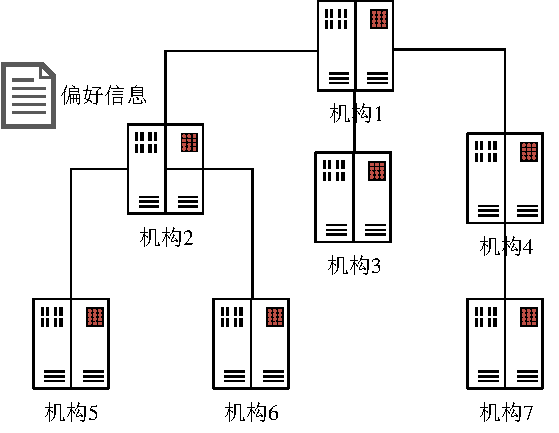
\includegraphics[width=350pt]{jigou_tree.pdf}
    \caption{机构部门间的树形关系}
    \label{jigoushu}
\end{figure}

另一方面,同一机构内部可能具有多个可提供计算能力的单位,他们具有相同的原位计算数据访问权,但他们的计算能力、质量又是参差不齐的。当同一机构内部的不同计算单位作为参与者进入到原位计算任务$T$的竞争环节中时,多个参与者可能提供的是数据相同而计算方式或者服务质量具有差异的原位计算。相同的计算内容对于同一原位计算任务$T$来说是冗余的。因此在前述场景中,这些数据同质的参与者之间实质存在互斥关系。即在这些数据同质的参与者中,分配规则最多只能选择1个胜出者。同一机构可能拥有多个不同的数据源,因此在一家机构内部也可能存在多组这样的互斥关系。目前我们只考虑在来自一家机构的参与者中存在数据同质的现象。
\begin{figure}[h]
    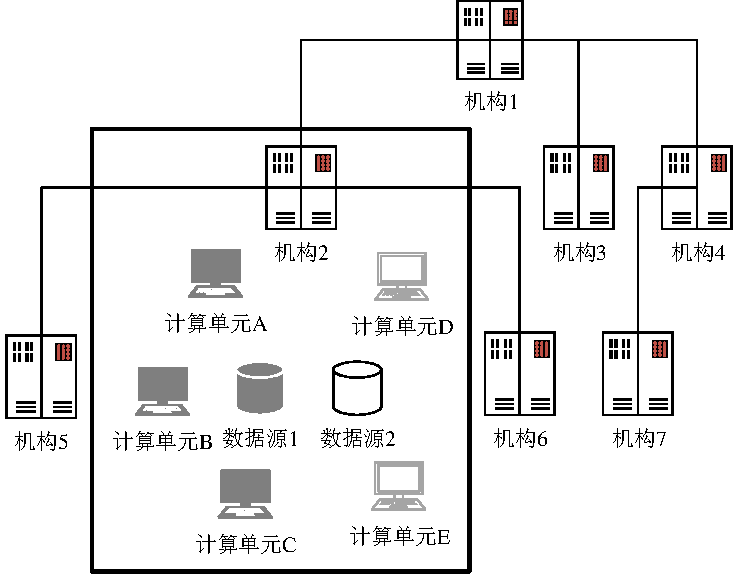
\includegraphics[width=350pt]{huchi_tree.pdf}
    \caption{机构内部参与者的互斥关系示例}
    \label{huchishu}
\end{figure}

在图\ref{huchishu}的示例中,机构2的计算单元$A,B,C$拥有数据源$1$的访问权,计算单元$D,E$拥有数据源$2$的访问权。当这些计算单元参与至原位计算任务竞争环节时,计算单元$A,B,C$及$D,E$中各自最多只能有一个胜出者。
\subsubsection{形式化}

在前文的形式化定义中增加机构的概念。机制中共有$m$个机构,所有参与者$agent_i,1 \leq i \leq n$隶属于这些机构。每个机构具有参与者偏好$prefer_i$,描述了其对自身管辖的部门参与原位计算的限制条件。现仅考虑如下限制:该机构及其管辖部门的参与者所提供的总原位计算任务不能超过$limit_i$单位。此节的分析及结论可以被推广至所有限制指标$\leq$某一阈值的更一般情况。机构之间形成森林结构,即对于$org_i$,其最多仅有一个父亲节点。

$agentpinorg_i=\{agent_k|agent_k属于机构i\}$是隶属于机构$orgs_i$的参与者集合。该集合可以根据参与者对数据源的依赖关系被划分为$datasourcenum$个子集,每个子集最多产生一名胜出者。

\subsection{问题求解}
为森林状的机构添加虚根,使其转为树形结构。然后将上述场景抽象成图\ref{chouxiangtree}。其中圆形代表机构,三角形代表机构中的计算单元,即机制的参与者。颜色的不同体现了其数据来源的差异性,从而将他们划分为不同的互斥组。此时的社会福利最大化问题解决思路与前两节相似,不同点在于动态规划需要在整个树形结构上进行。

\begin{figure}[h]
    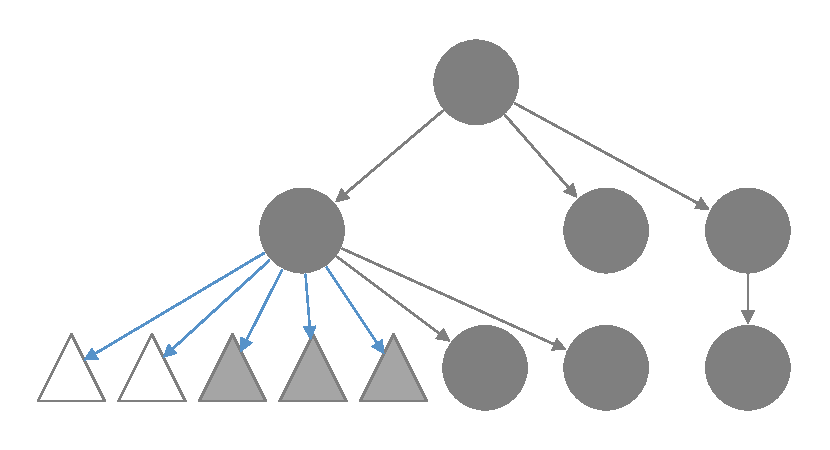
\includegraphics[width=350pt]{chouxiangtree.pdf}
    \caption{树形结构抽象图}
    \label{chouxiangtree}
\end{figure}

仿照方程\ref{dpfangcheng}拟定6维状态$dp[i,j,a,b,c,t]$,表示考虑第$i$个机构,刚好分配$j$单位原位计算任务,其中一级参与者$a$个,二级参与者$b$个,三级参与者$c$个,最多花费$t$单位总时间,所能够获得的最大收益。
所能够获得的最大收益。

由泛化物品的概念可知,每一个状态可以理解为一个泛化物品。那么原状态转移则是这些泛化物品在树上自底向上不断求和的过程。值得注意的是,图\ref{chouxiangtree}中每个机构所属的三角形(计算单元)首先要根据其互斥关系,以动态规划的方式合成一个泛化物品,然后再参与到树上的泛化物品合并流程。在此过程中同时记录最优路径。

另一方面,各个机构的偏好$prefer_i$也可以在树上最优化的过程中解决。树上最优化流程进行到机构i时,他可以直接将状态$dp[i,limit_i+1...datademand,,,,]$全部置为非法状态。然后沿着树形结构继续最优化过程。本场景中的问题求解思想与\ref{dptou}节中的思想是一致的。故此处直接给出分配规则。

\begin{algorithm}[H]
\KwIn{$\mathbf{datacount,timeperunit,level,bid},datademand$,\ref{dpdingyi}节中定义的限制指标,本节新定义的量}
    \KwOut{$\mathbf{allocation}$}
    $generalizeditem(\text{虚根},datademand,parti_1,parti_2,parti_3,TIME)$\;
    以最优路径对$\mathbf{allocation}$进行赋值。\;
\;
\;
    $generalizeditem(i,j,a,b,c,t)$定义为:\;
    
    \eIf{i具有计算单元,即$agentpinorg_i \neq \emptyset$}
    {
        以其计算单元的信息运行算法思想\ref{jiyihua},注意同一组内最多选取一个参与者分配计算任务,得到泛化物品$init$\;
        记录最优路径\;
    }{
        $init$是一个不产生任何影响的初始泛化物品。
    }
    \For{机构i的每一个下属单位u}
    {
        计算$generalizeditem=(u,0...datademand,0...parti_1,0...parti_3,0...parti_3,0...TIME)$,得到泛化物品u\;
        将泛化物品u并入$init$\;
        \tcp{按照既定的优先级处理多解的情况}
        记录最优路径\;
    }
    将$init[,limit_i+1...datademand,,,,]$中的所有状态置为非法状态\;
    \Return $init$\;
\caption{树形场景下的分配规则}
\label{tree_allocation}
\end{algorithm}

算法\ref{tree_allocation}中,时间复杂度较高,约为$O(m*S^2)$,$S$为除第一维状态以外的五维子空间的总状态数。其关键步骤在于泛化物品之间的和并,思想是直接枚举费用状态在两者之间的分配。

\begin{theorem}
 算法\ref{tree_allocation}所示的分配规则仍然单调。 
\end{theorem}

\begin{proof}
证明思想与\ref{dpdandiao} 完全一致
\end{proof}

由于互斥组的存在,动态规划的无后效性被破坏,难以像前文一样直接将$agent_i$移至末位,然后算出各个阶跃值。当然,若为每个互斥组增加一维二值状态,仍然可解,但此时的状态空间大小似乎难以接受。接下来直接以二分查找的方式来寻找这些阶跃值,时间复杂度为$O(allocation_i*log(INCENT))$。若$bid_i$的范围较小,也可以直接枚举求解。应根据具体数据量做相应调整。

\begin{algorithm}[H]
\KwIn{$\mathbf{datacount,timeperunit,level,bid},datademand$,\ref{dpdingyi}节中定义的限制指标,本节新定义的量}
    \KwOut{$\mathbf{payment}$}
    运行算法\ref{tree_allocation},得到$\mathbf{allocation}$\;
    \For{每个$agent_i$}
    {
        $payment_i \leftarrow 0$\;
        \For{$ks \leftarrow 0$ \KwTo $allocation_i$}
        {
            二分$bid_i$,运行算法\ref{tree_allocation},找到$allocation_i = ks$的临界标的$b$。
            $payment_i \leftarrow payment_i + b$
        }
    }
\caption{树形场景下的支付规则}
\label{tree_zhifu}
\end{algorithm}

\section{本章小结}
在简单可并行计算场景下,本文中的竞争拍卖机制设计部分依次讨论了基础模型、多重指标限制、场景扩展及额外偏好等议题。基础模型是拍卖机制的基础部分。在有限理性人、准线性效用等假设下,分配规则为满足任务方数据量需求和参与者数据限制条件下的社会福利最大化。多重指标限制引入了任务方对待分配的原位计算任务的进一步细节要求。例如:时效性,参与者数量,信誉评级等。而场景扩展及额外偏好更进一步考虑了参与者的上下级关系带来的新的偏好限制,以及数据同质参与者之间的互斥性。以上三种机制均满足社会福利最大化、DSIC。基础模型可以在多项式时间内求解,而多重指标限制和场景扩展及额外偏好需要在伪多项式时间内求解。

\chapter{计算依赖相关的机制设计}
\section{引言}
\section{基础场景}
\subsection{问题描述及定义}
原位计算环境中,由于任务$T$对数据依赖的内在复杂性,数据分布的差异性等因素,更一般的情形是计算不可分布式并行完成。此时,原计算任务$T$被分割算法根据所需数据划分为若干个更小的计算子任务。每个子任务满足原位计算的限制,即其计算仅依赖于本地数据。然后合并算法将这些子任务的计算结果重新合并成原始计算问题$T$的解。而合并的结果的方式并不单一,可能包含了若干次迭代操作。这些反复的结果传输带来的时延会造成总计算时间增加。这是分布式计算环境不可避免的问题。而另一方面,参与原位计算的各个节点的计算能力可能有较大差异。若是将子任务分配给了效率极低的计算节点,原位计算的时效性将会进一步降低。这对于响应时间敏感的计算任务而言是难以接受的。因此,本章主要以时间限制来分析计算依赖相关的机制设计问题。

\subsubsection{形式化定义}
对于计算任务$T$,分割算法将其划分为子任务集合$\mathbf{SubTask},|\mathbf{SubTask}| = ST$。这些子任务之间的同步存在拓扑序关系。为了描述这种关系,我们借用AOE网的思想。构建有向无环图$D=(\mathbf{V},\mathbf{E})$,集合$\mathbf{V}$是所有同步节点的集合。有向边$<u,v> \in \mathbf{E}$表示子任务的进行。另有关于有向边的函数$t(e)$,其值是子任务$e$由该任务的胜出者进行计算所需时长。每个子任务$SubTask_i$拥有竞争该任务的参与者列表$list_i$,每个参与者$agent_{ij} \in list_i$有关于任务$SubTask_i$的私密估值$val_i$以及其完成该计算任务所需时间$timefromagent_i$。每个列表中只能产生也必须产生一名胜出者,来完成该子任务的计算。此处假定所有参与者仅参与一项子任务的竞争。最重要的限制条件是:所有子任务的胜出
者确定后,总任务的完成时间$finishedtime \leq $某一阈值$timelimit$。包括效用函数、社会福利等其余定义与假设均与第三章类似,此处不做赘述。

\subsection{模型分析及求解}
\begin{figure}[h]
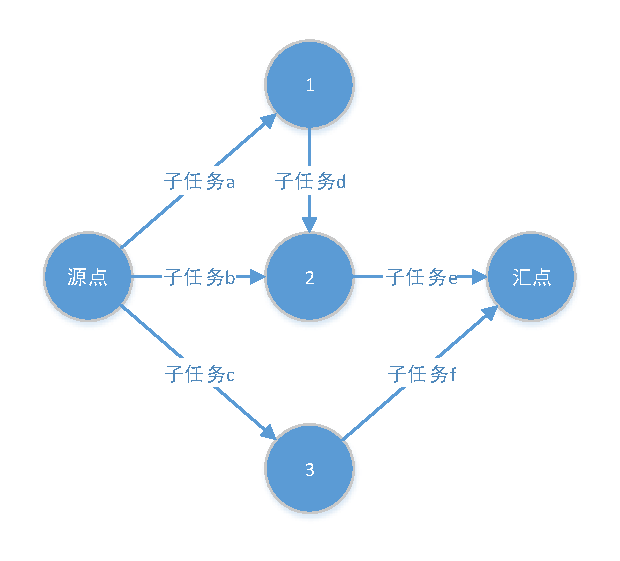
\includegraphics[width=350pt]{zirennwu_aoe.pdf}
\caption{子任务的AOE网示例}
\label{zirennwu_aoe}
\end{figure}

如图\ref{zirennwu_aoe}所示,每个顶点意味着子任务的同步等待。只有当指向该节点的所有边上所示子任务均完成时,同步等待方结束,继续进行后续子任务计算。给定$AOE$网,可以利用关键路径算法求出该网络的最少花费时长。对于图\ref{zirennwu_aoe}中的顶点$i$,同步等待结束当且仅当其所有前驱顶点等待结束且对应边上的子任务完成。而顶点$i$结束等待所需花费的时长是其所有前驱花费时长与对应子任务时长之和的最大值。此时产生明显的最优子结构,而在DAG中,这些子结构是会被重复求解的。
拟定状态$dp[i],1 \leq i\leq |V|$,表示同步节点$i$完成等待所需的时间。则有转移方程$dp[i] = max(dp[k]+t(<k,i>)|<k,i> \in \mathbf{E}),dp[\text{源}] = 0$。总任务所需时间$finishedtime$即为$dp[\text{汇}]$。

假设所有参与者已经真实地表达对各自计算子任务的估值,并给出标的,即$\mathbf{bid}=\mathbf{val}$。此时社会福利最大化可以形式化问题\ref{jichumoxing2}。
\begin{align}
    \label{jichumoxing2}\max_{\vec{allocation}} \quad&\sum_{i=1}^{n}{bid_i*allocation_i}\\
    s.t                     \quad&allocation_i = \{0,1\}\notag\\
    \quad&\left(\sum_{i=1}^{n}{I(agent_i \in list_j)*allocation_i}\right) = 1,\text{for every }1 \leq j \leq ST\notag\\
    \quad&finishedtime(\mathbf{allocation}) \leq timelimit
    \notag
\end{align}

考虑$SubTask_i$的胜出者选择过程,对于参与者$i,j$,若$val_i < val_j$,且$timefromagent_i > timefromagent_j$,则$agent_i$完全劣于$agent_j$,故可以将$allocation_i$直接置为0。此时可以认为,$timefromagent$随着$val$单调递增。这意味着选取更大估值的参与者会带来更长的计算时长,在$AOE$网中,若该子任务对应的边在关键路径上。那么会引起总的时长增加,可能违反限制条件。总体来看,假设每条边共有$a$种选择(对应于该子任务的$a$个竞争者),那么$b$条边,总可行集大小就有$a^b$种,似乎难以接受。

\begin{theorem}
   问题\ref{jichumoxing2}属于NP-hard问题。
\end{theorem}

\begin{proof}
    令$S$表示问题\ref{jichumoxing2}。要证$S\in NP-hard$,需要存在一个现有NPC问题$S'$归约至$S$。此处以0-1背包作为$S'$。

    对于$S'$的任意实例$ins$,共有$n$\footnote{此处的变量名仅在本证明内有效}个物品,n维向量$\mathbf{size}$和$\mathbf{val}$分别是物品质量向量和价值向量。$B$是背包容量。构建有向图$D=(\mathbf{V},\mathbf{E})$,$\mathbf{V} = {1,2,...,n,n+1},\mathbf{E} = \{(i,i+1)|1 \leq i \leq n\}$。对于$1 \leq i \leq n$,构建$list_i$,有两个参与者,$(timefromagent,bid) = \{(size_{i-1},val_{i-1}),(0,0)\}$。$timelimit = B$。得到问题\ref{jichumoxing2}的一个实例$ins'$。

    原问题$ins$的最优化等价于现问题$ins'$的求解。故任意0-1背包问题实例都可以在多项式时间内归约至问题\ref{jichumoxing2}的一个实例。故$S\in NP-hard$。
\end{proof}

由于问题\ref{jichumoxing2}是难以在多项式时间内精确求解的。本文研究一种贪心算法对其在伪多项式时间内进行近似求解。

贪心的思想是从初始可行解$S$开始,每次寻找一个满足时间限制条件的更优解$S'$取代原可行解,直到时间限制无法满足为止。

\begin{algorithm}[H]
    \KwIn{前文形式化定义的所有相关量}
    \KwOut{$\mathbf{allocation}$}
    对于任意子任务竞争列表中的任意参与者$i,j$,若$val_i < val_j$,且$timefromagent_i > timefromagent_j$,置$allocation_i = 0$,并将参与者$i$从该竞争列表中删除。然后将各个竞争者列表$list_i$中的参与者各自按照$timefromagent$关键字递增排序。\;

    初始化解$S$,其中所有子任务的胜出者为各自竞争列表中时长花费最小的参与者。\;
    若以$index_i$表示子任务$i$的当前胜出者在$list_i$中的下标。则$index_i = 1$。\;
    根据转移方程$dp[i] = max(dp[k]+t(<k,i>)|<k,i> \in \mathbf{E}),dp[\text{源}] = 0$计算$S$所需时间$ftime = dp[\text{汇}]$。\;
    \If{ftime > finishedtime}
    {
        任务无法在给定时限内完成,输出错误信息。\;
    }
    \While{True}
    {
        选出$\{bid_{index_i+1}-bid_{index_i}/timefromagent_{index_i+1}-timefromagent_{index_i}\}$中的最大值所对应的子任务下标j。\;
        构造新的解$S' = S$,除了$index_j = index_j+1$\;
        根据上述状态转移方程计算解$S'$是否满足时间限制条件。\;
        \If{$S'$不是可行解}
        {
            continue\;
        }
        $S = S'$\;
    } 
    根据最终解$S$中的胜出者确定分配向量$\mathbf{allocation}$\;
\caption{贪心近似求解计算依赖相关的问题}
\label{jichumoxing2tanxin}
\end{algorithm}

算法\ref{jichumoxing2tanxin}的思想是从最小社会福利的解开始,每次选择一个子任务$j$,该子任务选择更优胜出者的价值收益与时间花费损失的比值最大。然后判断新的解是否满足最长路时间限制条件。若新解是可行解则更新。否则当前解为此贪心算法下的最优解。算法时间复杂度为$O(|V|*n)$,n为总的参与者数量。由于总DAG是连通图,则$|V|- 1\leq |E|$,且$|E| = ST$。则时间复杂度约为$O((ST+1)*n)$,ST为子任务的数量。

\begin{theorem}
    算法\ref{jichumoxing2tanxin}所示分配规则$allocation_i(z,\mathbf{bid_{-i}})$不一定关于$agent_i$的标的$z$的单调不减。
\end{theorem}

\begin{proof}
    要证上述分配规则不一定单增,可以举一反例说明。一实例如图所示,共有两个串行的子任务,每个子任务有$3$个竞争的参与者。$list_1=\{(1,1),(2,3),(3,5)\},list_2=\{(1,1),(2,2),(3,9)\}$,二元组$(a,b)$表示$timefromagent=a,bid=b$,$timelimit=5$。运行算法\ref{jichumoxing2tanxin},可知$(2,2)$对应的参与者为胜出者之一。

    此时将$(2,2)$对应参与者$agent_z$的标的增加至$4$,即用$(2,4)$替代原$(2,2)$,再次运行算法\ref{jichumoxing2tanxin}。新的胜出者是$(3,9)$。因而对于$agent_z$来说,其分配函数并非关于其标的$bid_z$单增。
\end{proof}

更一般的可知,这种从初始状态开始,每一步选取选择下一个参与者的收益增量最大的子任务进行阶段性迭代更新的贪心策略对应的分配函数均不满足单增的性质。因为总是存在前述证明中的参与者$agent_z$的情况。由麦尔森引理及DSIC机制的必要条件可知此类贪心策略无法实施。

接下来考虑每次直接选择标的最大的参与者作为胜出者的贪心策略。
\begin{algorithm}[p]
    \KwIn{前文形式化定义的所有相关量}
    \KwOut{$\mathbf{allocation}$}
    对于任意子任务竞争列表中的任意参与者$i,j$,若$val_i < val_j$,且$timefromagent_i > timefromagent_j$,置$allocation_i = 0$,并将参与者$i$从该竞争列表中删除。然后将各个竞争者列表$list_i$中的参与者各自按照$timefromagent$关键字递增排序。\;

    初始化解$S$,其中所有子任务的胜出者为各自竞争列表中时长花费最小的参与者。\;
    
    根据转移方程$dp[i] = max(dp[k]+t(<k,i>)|<k,i> \in \mathbf{E}),dp[\text{源}] = 0$计算$S$所需时间$ftime = dp[\text{汇}]$。\;
    \If{ftime > finishedtime}
    {
        任务无法在给定时限内完成,输出错误信息。\;
    }

    对于所有参与者$agent_i$,其拥有二元组$(bid,timefromagent)$\;
    \tcp{(a,b)是$agent_i$所在竞争列表中时长花费最小的参与者对应的二元组信息}
    init $lst =\{(bid_i-a,timefromagent_i)\}$\;

    置所有子任务为未访问状态。\;

    \While{$lst$不为空}
    {
        根据第一关键字选出$lst$中的最大值对应的参与者$agent_k$。\;
        然后在$lst$中删除参与者$k$\;
        \If{参与者$k$对应的子任务$SubTask_u$已经被访问过}
        {
            continue\;
        }
        构造新的解$S' = S$,$agent_k$是$SubTask_u$的胜出者。\;
        根据上述状态转移方程检查解$S'$是否满足时间限制条件。\;
        \If{$S'$不是可行解}
        {
            continue\;
        }
        $S=S'$\;
        置$SubTask_u$为已被访问状态。\;
    }
    根据最终解$S$中的胜出者确定分配向量$\mathbf{allocation}$\;
\caption{贪心近似求解计算依赖相关的问题2}
\label{jichumoxing2tanxin2}
\end{algorithm}
类似的,最坏时间复杂度为$O(n*|V|)$,n为参与者数量。接下来说明分配规则的单调性。

\begin{theorem}
对于任意参与者$agent_i$以及任意$\mathbf{bid_{-i}}$,算法\ref{jichumoxing2tanxin2}所示分配规则$allocation_i(z,\mathbf{bid_{-i}})$是关于$agent_i$的标的$z$的单调不减函数。
\end{theorem}

\begin{proof}
记$al(z) = allocation_i(z,\mathbf{bid_{-i}})$,由前述场景可知,$al(z)\in\{0,1\}$。不妨假设$a<b,\text{且}al(a)=1$(对于$al(a)=0$的情况,$al(a)\leq al(b)$一定成立)。

对于$agent_i$并非其竞争列表中$timefromagent$值最小的情况,考虑算法\ref{jichumoxing2tanxin2}的流程,假设到$agent_i$之前根据标的递减排序的参与者序列为$p_1p_2p_3...p_k=agent_i$,若增大标的$z$会将$agent_i$的位次提前。在$z=b$的情况下,假设新的参与者序列为$p_1p_2p_3...p_u=agent_i...p_{k-1}p_{k+1}$。当贪心算法考虑到$p_u$时,由于$u<k,\text{且}al(a)=1$,$agent_i$所属子任务$SubTask$一定未曾被访问过。算法\ref{jichumoxing2tanxin2}中的新解$S'$也一定是可行解。否则,$al(a) = 0$。(因为算法确定序列$p_{u+1}...p_{k-1}$中新的胜出者的过程只会使得DAG的总时长不减少)。故$agent_i$会继续成为其所属子任务的胜出者,$al(a)\leq al(b)=1$。

若$agent_i$是其所属子任务的竞争列表中时长花费最小的参与者,增大$z$可能会使得部分后继参与者直接因绝对次优性被删除。而留下来的参与者的相对标的$bid_k - z$会减少,这导致相应的参与者位次后移。类似于前面的分析,这都不会改变$agent_i$的胜出者事实。故$al(a)\leq al(b)=1$始终成立。
\end{proof}
 
本场景下的分配向量$\mathbf{allocation}$被限制于0-1向量,故对于每个胜出者,只需找出其无法继续胜出的临界标的作为其支付的价格。算法\ref{jichumoxing2tanxin2zhifu}的最坏时间复杂度约为$O(|E|*(|V|+|E|)*(n+max(|E|,|E|*C)))$,$C\leq n$为各个子任务对应参与者数量的最大值。即为$O(|E|^2*n*(|V|+|E|))$,$n$为总参与者数量。

\begin{algorithm}[p]
    \KwIn{前文形式化定义的所有相关量}
    \KwOut{$\mathbf{payment}$}
    %\SetAlgoVlined
    执行算法\ref{jichumoxing2tanxin2},得到$\mathbf{allocation}$\;
    \For{每个$agent_i$}{
        \eIf{$allocation_i = 0$}
        {
            $payment_i = 0$\;
        }
        {
            
            将单减的原始相对标的序列$\mathbf{b}=b_1b_2b_3...b_k$中与$agent_i$属于同一竞争列表的所有相对标的$b_a,b_b,b_c,...,b_{agent_i},b_{next}...$全部删除,得到新的原始标的序列$\mathbf{b'}$\;
            使用$\mathbf{b'}$重新运行算法\ref{jichumoxing2tanxin2},得到各个胜出者产生时对应的图序列$\mathbf{GS}=G_1,G_2,G_3...G_u$,每个$G_i$是算法\ref{jichumoxing2tanxin2}中的一个新的可行解$S'$对应的DAG\;
            \eIf{$agent_i$的时长不是其竞争列表中最小的}
            {
                假设$agent_i$的相对标的$z$在图序列$\mathbf{GS}$中的位次是$G_1,G_2,...z,G_j,G_{j+1}....G_u$\;
                \For{$v = j $ \KwTo $ u$}
                {
                    在$G_v$的基础上将$agent_i$置为所属子任务的胜出者,得到新解$S'$,以算法\ref{jichumoxing2tanxin2}中最长路的计算方法检查$S'$的合法性\;
                    \If{$S'$不合法}
                    {
                        $payment_i = bid_i + max(G_v\text{所对应的相对标的},agent_i\text{后一位的相对标的}b_{next}) -$ $agent_i$的相对标的$z$\;
                        break\;
                    }
                }
            }{

                假设与$agent_i$所属同一子任务的其余相对标的在图序列$\mathbf{GS}$中的位次是$G_1,G_2,...,z_1,...,z_2,...,z_k,...G_u$。不断减少$bid_i$,直到$z_1,...z_k$中首次出现新的胜出者,减少量为$\Delta b$\;
                \eIf{$\Delta b > bid_i$}
                {
                    $payment_i = 0$\;
                }
                {
                    $payment_i = bid_i - \Delta b$\;
                }

            }
        }
    }
\caption{贪心近似求解计算依赖相关的问题2支付规则}
\label{jichumoxing2tanxin2zhifu}
\end{algorithm}



%考虑在参与者对各子任务的估值及相差不多的情况下,此时DAG中长路相较于短路应当提供更多的价值贡献。因而可以优先确定长路上的规划问题的解%,然后再考虑较短路上的规划问题。

%拟定二维状态$dp[i,w]$表示单链的规划过程中,本链上节点$i$的前驱子任务在时间$w$内依次完成,所获得最大价值。则有状态转移方程\ref{%dpfangchengdanlian}

%
%\begin{gather}
%\label{dpfangchengdanlian}
%dp[i,w] = \max_{agent_k \in list_{<j,i>}}{dp[j,w-timefromagent_k]+bid_k},j\text{是}i\text{在本链上的前驱节点}
%\\
%dp[\text{源}][0...timelimit] = 0 \notag
%\end{gather}

%
%\begin{algorithm}[H]
    %\KwIn{前文形式化定义的所有相关量}
    %\KwOut{$\mathbf{allocation}$}
%    对于任意子任务竞争列表中的任意参与者$i,j$,若$val_i < val_j$,且$timefromagent_i > timefromagent_j$,置$allocation_i = 0%$,并将参与者$i$从该竞争列表中删除。\;

%    %

    %inital dp[|V|][timelimit]\;

%\caption{changluyouxian}
%\label{tree_zhifu}
%\end{algorithm}

%
%不妨从另一个角度来考虑该问题。若有向边$<u,v>$上的权值发生改变,仅会影响节点$v$及其后继节点的完成同步等待时间,而对节点$u$及其前驱节点无影响。这呈现明显的最优子结构及无后效性:每条边上的胜出者选择可以看做是阶段性决策,该阶段的决策不受后继节点决策影响,仅依赖于前%驱的决策状态。

%//
%拟定二维状态$dp[i,w],1 \leq i \leq |V|,0 \leq j \leq timelimit$,表示节点$i$的前驱边全部确定胜出者,且节点$i$%完成同步等待的总时间不超过$j$时,所获得的最大价值。状态转移方程如\ref{dpfangcheng2}所示。

%\begin{gather}
%\label{dpfangcheng2}  
%dp[i,w] = \sum_{<j,i>\in \mathbf{E}}{\max_{agent_k \in list_{<j,i>}}{dp[j,w-timefromagent_k]+bid_k}}
%\\
%dp[\text{源}][0...timelimit] = 0 \notag
%\end{gather} 
%//



\section{最优拍卖机制设计}

在前文的机制设计中,平台方根据定义好的社会福利来确定分配规则及价格规则,对应于社会福利最大化问题。这样的分配规则可以使得系统整体收益最优,但此时平台方的收益无法确切保证。若平台方的预算是有限的,则需要设计新的分配规则及价格函数来保证平台方的利益。由\ref{jichumoxingdingyi}节可知,平台方的真实收益是$profit = \sum_{i}^{n}{payment_i}-m*INCENT$,其中$m$是原位计算任务$T$所需单位计算的数量。在简单可并行场景下,$m=datademand$;在计算依赖相关场景下,$m=ST$。$-m*INCENT$部分是固有值,不可更改。最大化$profit$等价于最大化$\sum_{i}^{n}{payment_i}$。本节采用期望税收最大化的机制设计来保证平台方在平均意义下的收益最优。

\subsection{模型假设}

现有独立的概率分布$F_1,F_2,F_3,...F_n$及对应的连续概率密度函数$f_1,f_2,f_3...f_n$,且这些分布均存在有限期望。参与者$agent_i$的私密值$val_i$的概率分布是$F_i$。

\subsection{分析及求解}
虚拟估值定义为$\varphi _i(v_i)=v_i-\frac{1-F_i(v_i)}{f_i(v_i)}$。在参与者真实得给出标的的情况下,期望税收等于期望虚拟社会福利。即

\begin{equation}
    \mathbf{E}_{\mathbf{v}\sim\mathbf{F}}{\left[\sum_{i}^{n}{payment_i(\mathbf{v})}\right]}=\mathbf{E}_{\mathbf{v}\sim\mathbf{F}}{\left[\sum_{i}^{n}{\varphi _i(v_i)*allocation_i(\mathbf{v})}\right]}
\end{equation}

故期望税收最大化等价于期望虚拟社会福利最大化。考虑场景\ref{jichumoxing2},虚拟社会福利最大化仍然是$NP-hard$问题,故仍采用算法\ref{jichumoxing2tanxin2}近似求解。而为了满足参与者真实投标的前提,需要讨论虚拟社会福利最大化对应分配函数$virtualal$的单调性。

\begin{algorithm}[H] 
    \KwIn{形式化定义的所有量}
    \KwOut{$\mathbf{allocation}$}
    将所有参与者的标的$bid_i$以其虚拟估值$\varphi _i(bid_i)$替代\;
    其它信息不更改,运行算法\ref{jichumoxing2tanxin2},得到$\mathbf{allocation}$\;
\caption{最优拍卖机制分配规则}
\label{optimalauction}
\end{algorithm}



\begin{theorem}
若任意分布的失效率函数$\frac{f_i(v)}{1-F_i(v)}$关于$v$单调不减,则对于任意参与者$agent_i$以及任意$\mathbf{bid_{-i}}$,算法\ref{optimalauction}所示分配规则$allocation_i(z,\mathbf{bid_{-i}})$是关于$agent_i$的标的$z$的单调不减函数。
\end{theorem}

\begin{proof}
虚拟社会福利可能引入的负数标的不影响原问题求解。算法\ref{jichumoxing2tanxin2}所示分配规则单调不减,若分布的失效率函数单调不减,则虚拟估值$\varphi _i(v_i)$单调不减,则$allocation_i(z,\mathbf{bid_{-i}})$也单调不减。
\end{proof}

类似地,给出最优拍卖的支付规则。

\begin{algorithm}[H] 
    \KwIn{形式化定义的所有量}
    \KwOut{$\mathbf{payment}$}
    将所有参与者的标的$bid_i$以其虚拟估值$\varphi _i(bid_i)$替代\;
    运行算法\ref{jichumoxing2tanxin2zhifu},得到$\mathbf{payment}$\;
    \For{$allocation_i=1$的参与者}
    {
        将$payment_i$替换为$\varphi _{i}^{-1}{payment_i}$
    }
\caption{最优拍卖机制支付规则}
\label{optimalauctionzhifu}
\end{algorithm}



\section{本章小结}

\chapter{面向数据价值共享的激励机制设计与实现}
\section{实验概述}
\section{总体设计}
\section{模块设计}
\section{界面展示}
\section{本章小结}

\chapter{全文总结与展望}

\section{全文总结}
本文以时域积分方程方法为研究背景,主要对求解时域积分方程的时间步进算法以及两层平面波快速算法进行了研究。


\section{后续工作展望}
时域积分方程方法的研究近几年发展迅速,在本文研究工作的基础上,仍有以下方向值得进一步研究:

\thesisacknowledgement
在攻读硕士学位期间,首先衷心感谢我的导师XXX教授


\nocite{*}
\thesisloadbibliography{reference}

%
% Uncomment following codes to load bibliography database with native
% \bibliography command.
%
% \nocite{*}
% \bibliographystyle{thesis-uestc}
% \bibliography{reference}
%

\thesisappendix

\chapter{中心极限定理的证明}

\section{高斯分布和伯努利实验}

\thesisloadaccomplish{publications}


\thesistranslationoriginal
\section{The OFDM Model of Multiple Carrier Waves}


\thesistranslationchinese

\section{基于多载波索引键控的正交频分多路复用系统模型}

\end{document}
